\begin{pastexam}[label={px:ntu-109-comm-dsa-43}]{臺大電信所 109 學年度（B）第 43 題}
（複選；每題 2 分，每答錯一個選項倒扣 0.4 分）

Consider the expression tree in Fig.1
\begin{enumerate}[label=(\Alph*),nosep]
\item The prefix expression is \texttt{a+b*c+d+e*f*g*h+i+j*k}
\item The prefix expression is \texttt{*++a*bc*+def*g++hi*jk}
\item The infix expression is \texttt{*+*+*g+a*+f+*bcdehijk}
\item The postfix expression is \texttt{abc*+de+f*+ghi+jk*+**}
\item The postfix expression is \texttt{k*j+i+h*g*f*e+d+c*b+a}
\end{enumerate}

\begin{center}
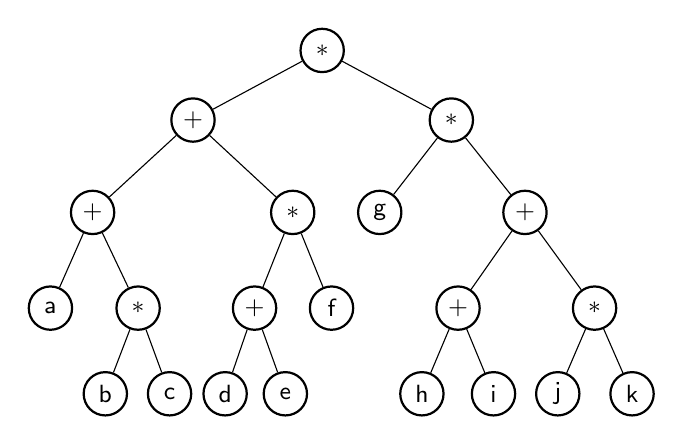
\begin{tikzpicture}[scale=0.85, v/.style={circle,draw,minimum size=5.5mm,inner sep=0pt,font=\small\sffamily,thick}]
\node[v] (r) at (5.36,-1.38) {$*$};
\node[v] (p1) at (3.43,-2.42) {$+$};
\node[v] (m1) at (7.29,-2.42) {$*$};
\node[v] (p2) at (1.93,-3.80) {$+$};
\node[v] (m2) at (4.92,-3.80) {$*$};
\node[v] (g) at (6.22,-3.80) {g};
\node[v] (p3) at (8.39,-3.80) {$+$};
\node[v] (a) at (1.30,-5.23) {a};
\node[v] (m3) at (2.61,-5.23) {$*$};
\node[v] (p4) at (4.35,-5.23) {$+$};
\node[v] (f) at (5.50,-5.23) {f};
\node[v] (p5) at (7.39,-5.23) {$+$};
\node[v] (m4) at (9.43,-5.23) {$*$};
\node[v] (b) at (2.12,-6.51) {b};
\node[v] (c) at (3.08,-6.51) {c};
\node[v] (d) at (3.91,-6.51) {d};
\node[v] (e) at (4.81,-6.51) {e};
\node[v] (h) at (6.85,-6.51) {h};
\node[v] (i) at (7.92,-6.51) {i};
\node[v] (j) at (8.88,-6.51) {j};
\node[v] (k) at (9.99,-6.51) {k};
\draw (r) -- (p1); \draw (r) -- (m1);
\draw (p1) -- (p2); \draw (p1) -- (m2);
\draw (m1) -- (g); \draw (m1) -- (p3);
\draw (p2) -- (a); \draw (p2) -- (m3);
\draw (m2) -- (p4); \draw (m2) -- (f);
\draw (p3) -- (p5); \draw (p3) -- (m4);
\draw (m3) -- (b); \draw (m3) -- (c);
\draw (p4) -- (d); \draw (p4) -- (e);
\draw (p5) -- (h); \draw (p5) -- (i);
\draw (m4) -- (j); \draw (m4) -- (k);
\end{tikzpicture}

Fig.1 Expression tree
\end{center}
\end{pastexam}

\begin{pastsoln}
答案：(B)(D)。

先把樹寫成加括號的中序式（資結書第~7.7~節），確認每個運算子的兩個運算元：
\[
\bigl((a + b * c) + (d + e) * f\bigr) * \bigl(g * ((h + i) + j * k)\bigr).
\]
根是 $*$，左子樹是 $(a + b*c) + (d + e)*f$，右子樹是 $g * \bigl((h + i) + j*k\bigr)$。

\textbf{前序}（根、左、右）：根 $*$；左子樹 $+\;+\,a\,{*}\,b\,c\;\;{*}\,{+}\,d\,e\,f$；右子樹
${*}\,g\;{+}\,{+}\,h\,i\;{*}\,j\,k$。 接起來是 \texttt{*++a*bc*+def*g++hi*jk}。

\textbf{後序}（左、右、根）：左子樹 \texttt{abc*+de+f*+}，右子樹 \texttt{ghi+jk*+*}，最後根
\texttt{*}，得 \texttt{abc*+de+f*+ghi+jk*+**}。

\textbf{中序}（不加括號）：\texttt{a+b*c+d+e*f*g*h+i+j*k}。

逐項：
\begin{itemize}
\item (A) 錯：這串是中序（而且沒有括號，運算順序已經和樹不同），不是前序。
\item (B) 對：和上面的前序一字不差。
\item (C) 錯：中序的第一個字元一定是最左邊的葉節點 $a$，不可能是運算子；這串不是任何一種
走訪。
\item (D) 對：和上面的後序一字不差。
\item (E) 錯：這是中序倒過來寫。 後序的最後一個字元必須是根 $*$。
\end{itemize}
\end{pastsoln}
